

%%%%%%%%%%%%%%%%%%%%%%%%%%%%%%%%%%%%%%%%%%%%%%%%%%%%%%%%%%%%%%%%%%%%
%% I, the copyright holder of this work, release this work into the
%% public domain. This applies worldwide. In some countries, this may
%% not be legally possible; if so: I grant anyone the right to use
%% this work for any purpose, without any conditions, unless such
%% conditions are required by law.
%%%%%%%%%%%%%%%%%%%%%%%%%%%%%%%%%%%%%%%%%%%%%%%%%%%%%%%%%%%%%%%%%%%%

\documentclass[
  digital, %% This option enables the default options for the
           %% digital version of a document. Replace with `printed`
           %% to enable the default options for the printed version
           %% of a document.
  table,   %% Causes the coloring of tables. Replace with `notable`
           %% to restore plain tables.
  lof,     %% Prints the List of Figures. Replace with `nolof` to
           %% hide the List of Figures.
  lot,     %% Prints the List of Tables. Replace with `nolot` to
           %% hide the List of Tables.
  %% More options are listed in the user guide at
  %% <http://mirrors.ctan.org/macros/latex/contrib/fithesis/guide/mu/fi.pdf>.
  oneside
]{fithesis3}
%% The following section sets up the locales used in the thesis.
\usepackage{listings}
\usepackage[resetfonts]{cmap} %% We need to load the T2A font encoding
\usepackage[T1,T2A]{fontenc}  %% to use the Cyrillic fonts with Russian texts.
\usepackage[
  main=english, %% By using `czech` or `slovak` as the main locale
                %% instead of `english`, you can typeset the thesis
                %% in either Czech or Slovak, respectively.
 %english, german, russian, czech, slovak %% The additional keys allow
]{babel}        %% foreign texts to be typeset as follows:
\usepackage{subfig}

\usepackage[                % Appendices
  toc,page
]{appendix}
%%
%%   \begin{otherlanguage}{german}  ... \end{otherlanguage}
%%   \begin{otherlanguage}{russian} ... \end{otherlanguage}
%%   \begin{otherlanguage}{czech}   ... \end{otherlanguage}
%%   \begin{otherlanguage}{slovak}  ... \end{otherlanguage}
%%
%% For non-Latin scripts, it may be necessary to load additional
%% fonts:
\usepackage{paratype}
\bibliographystyle{unsrt}
\usepackage{hyperref}
\usepackage[
   backend=biber        % if we want unicode
  ,style=numeric % or iso-numeric for numeric citation method
  ,autolang=other       % to support multiple languages in bibliography
  ,sortlocale=cs_CZ     % locale of main language, for sorting
  ,bibencoding=UTF8     % this is necessary only if bibliography file is in different encoding than main document
]{biblatex}
\usepackage{hyphenat}
\hyphenation{block-chain}
\def\textrussian#1{{\usefont{T2A}{PTSerif-TLF}{m}{rm}#1}}
%%
%% The following section sets up the metadata of the thesis.
\thesissetup{
    date          = \the\year/\the\month/\the\day,
    university    = mu,
    faculty       = fi,
    type          = mgr,
    author        = Tomáš Šíma,
    gender        = m,
    advisor       = {RNDr. Martin Stehlík},
    title         = {Darknet market analysis and user de-anonymization},
    TeXtitle      = {Darknet market analysis and user de-anonymization},
    keywords      = {blockhain, bitcoin, darknet, drug market, Tor, cryptocurrency, anonymity, metadata, de-anonymizatio
n},
    TeXkeywords   = {blockhain, bitcoin, darknet, drug market, Tor, cryptocurrency, anonymity, metadata, de-anonymizatio
n},
    abstract      = {
    
    We created a tool, which collects data from publicly available social networks and websites related to bitcoin(Twitter, Bitcointalk, Reddit,
    blockchain.info), online darknet market Valhalla and bitcoin blockchain.
    The tool imports these data to database, run multiple heuristics
    and provides user interface for visualizing data and metadata of addresses and identities related to 
    cryptomarkets and blockchain.
    The tool can for given bitcoin address find the nearest addresses or transactions related to Valhalla drug market
    or addresses that are mentioned in scraped websites. 
    
    To test the efficiency of this tool, we created two profiles on Valhalla cryptomarket and performed
    multiple transactions to deposit and withdraw bitcoins. We imported into tool the bitcoin addresses of
    the first profile recieved bitcoins from and checked, if the tool is able to identify,
    that addresses owned by second profile had been sending/recieveing bitcoin from Valhall market also.
    
    This thesis has two goals. The first goal is to perform quantitative statistical analysis of
    Valhalla cryptomarket. We scraped Valhalla cryptomarket website for information about vendors, listings and buyers
    and brought up a lot of interesting statistics about them.
    
    The second goal of this thesis is to create a tool to find, analyze and visualize publicly available data,
 which can be helpful to deanonymize users of drug markets available via Tor on dark web. The aim of this tool
 is to help investigators with collecting intelligence about entities related to these drug markets. Users and operators of these markets employ multiple means to prevent their deanonymization. Cryptomarkets are operated
 as Tor services, PGP encryption is often required to communicate between multiple parties and bitcoin is used as a way of paying for goods or services.
 
    },
    thanks        = {I would like to thank my supervisor RNDr. Martin Stehlík Ph.D. for guiding me and providing technical support for my work. 
    
    I would also like to thank Mgr. Jaroslav Šeděnka for his continuous stream of helpful comments and ideas.
    
    Access to computing and storage facilities owned by parties and projects contributing to the National Grid Infrastructure MetaCentrum provided under the programme "Projects of Large Research, Development, and Innovations Infrastructures
" (CESNET LM2015042), is greatly appreciated.},
    bib           = citations.bib
}

\usepackage{makeidx}      %% The `makeidx` package contains
\makeindex                %% helper commands for index typesetting.
%% These additional packages are used within the document:
\usepackage{paralist} %% Compact list environments
\usepackage{amsmath}  %% Mathematics
\usepackage{amsthm}
\usepackage{amsfonts}
\usepackage{url}      %% Hyperlinks
\usepackage{markdown} %% Lightweight markup
\usepackage{listings} %% Source code highlighting
\usepackage{graphicx}
\graphicspath{ {images/} }
\lstset{
  basicstyle      = \ttfamily,%
  identifierstyle = \color{black},%
  keywordstyle    = \color{blue},%
  keywordstyle    = {[2]\color{cyan}},%
  keywordstyle    = {[3]\color{olive}},%
  stringstyle     = \color{teal},%
  commentstyle    = \itshape\color{magenta}}
\usepackage{floatrow} %% Putting captions above tables
\usepackage{geometry}
\usepackage{pythontex}

\floatsetup[table]{capposition=top}
\begin{document}
\setpygmentsfv{xleftmargin=4ex}
\chapter{Introduction}
%\addcontentsline{toc}{chapter}{Introduction}

The relative anonymity of the Internet offers an incentive for criminal parties
to use the Internet as a toolG for their activities.
Internet facilitates some forms of existing crimes (selling drugs, guns and
counterfeits, running Ponzi schemes) and also enables many new types of frauds like hacking, phishing and identity theft.

Publicly available statistics show that cybercriminals are much
 less likely to be discovered and persecuted than criminals operating offline.
 In the USA in 2010, there were 5628 robberies and the loot was recovered in more than 20\% cases. \parencite{fbi10} 
 In the same year FBI recieved 303809 complaints related to cyber crime, resulting in just 6 convictions. \parencite{fbcyber} 
Criminals value their anonymity very highly and use various means to prevent being caught by police forces.
\parencite{tzanetakis2016transparency}
\parencite{van2013surfing}
\parencite{aldridge2014not}

A big problem for criminals was getting the money they got from criminal activity to their possession,
since that required some form of physical presence or identification.
Also, it was hard for two anonymous entities engaging in criminal activity to transfer value to each other,
 because it's hard to set up an anonymous bank account and neither party could be sure about the origin of
 the money they have received.

For bitcoin, there is no central authority requiring bitcoin address
(bitcoin equivalent of bank account number) to be linked to person's identity and so 
criminals can just use their connection to the Internet to both receive and send bitcoins without disclosing their identity.
However, all bitcoin transactions are publicly available and so each bitcoin can be tracked through the whole transaction history.

 Cryptomarkets are online marketplaces, where vendors offer illicit goods and services.
 Cryptomarkets are accessible via Tor network as an .onion service, users of
 cryptomarkets use PGP to communicate with each other and use bitcoin as a way to transfer value.
These mechanisms make it possible for cryptomarkets to publicly operate, yet be hard to reach by law enforcement.
\parencite{cox2016staying}

We scraped and examined data from Valhalla market,
 to our best knowledge one of the most popular and well established currently (February 2018) operating drug markets,
in order to do a statistical analysis of the scale of its operations.

All the bitcoin transactions are stored in blockchain. Blockchain is
publicly available, and so anyone can access data about bitcoin transactions.
Bitcoin transactions transfer bitcoins between bitcoin addresses. It is common practice for users
to generate new bitcoin address for each incoming transaction.
When user pays via bitcoin, he might use bitcoins just from some small subset of his bitcoin addresses
and so the recipent doesn't know about sender's addresses that were not used in the transaction.
This mechanism helps sender not disclose how many bitcoins he owns in total and also
protect reciever from finding all transactions that were done by sender in the past.

\section{Goals}

We created a toolchain for drug market users deanonymization by using publicly known data.
The tool imports bitcoin blockchain into neo4j graph database in order to create a graph of transactions.
It than runs multiple heuristics over this graph to cluster addresses that belong to the same user.
The tool scrapes multiple public sources related to drug markets and bitcoin transactions in order
to obtain some form of identification(username) linked to bitcoin address and adds this information to database.
It provides GUI where user can insert address and the program finds addresses with linked identities
that are few transactions away from the inserted address in the transaction graph.
We also created multiple scripts for scraping information about trades from Valhalla market website
and export them to .csv files and used these data for quantitative analysis of Valhalla market operations.

XXX - tool byl uspesny v detekovani tolika a tolika adres z pouzitych uctu, viz kapitola verifikace

\section{Structure of the thesis}
Chapter \emph{related terminology} starts with a quick introduction
on how cryptomarkets work and the technology they use.
It continue with describing the major technologies used by cryptomarkets -- bitcoins, Tor and PGP.
Chapter \emph{Related work} gives an overview of previously published works on similar topics. 

The chapter \emph{Methods and tools of data retrieval and analysis} describes the process of collecting
and storing the data from bitcoin blockchain, drug markets and publicly available forums and social networks. 

The chapter called 
\emph{Application for searching nearby identified addresses}
describes the functionality, architecture and implementation of the application that was created as part of this work.

Chapter \emph{Statistics of Valhalla cryptomarket} consists of various statistics about
drug markets that were gathered by Valhalla market website scraping.

\emph{Testing and verification} chapter is about the testing of the created application.
The last chapter is a discussion about achieved goals, problems of implementation and possible future improvements.

Chapter \emph{Conclusions and future work} discuss achieved goals and possible future extension and development
of this work.


\chapter{Related terminology}

In this chapter, I explain the terms and technology related to online drug markets.
Online drug markets use several technologies that are crucial to their anonymous operation.
Bitcoin enables different parties to exchange value in an anonymous way.
Tor allows users and administrators of a marketplace to hide from any third party doing packet sniffing on the network,
that they are accessing drug marketplace. It also hides the location on drug marketplace web server from its users.
PGP enables sellers and vendors to communicate between each other in an encrypted way,
so that drug market administrators cannot eavesdrop on that communication.

\section{Cryptomarkets}

Illegal online markets have been around for more than 30 years \parencite{motoyama2011analysis}.
On these markets, users can sell and buy drugs, weapons, hacking tools, stolen credit cards,
counterfeit currency, forged documents and other illegal goods and services.
Most markets forbid selling the most unambiguously harmful goods, such as child pornography or hitman services.

In 2011 there appeared a new type of illegal online marketplace called cryptomarket. 
A cryptomarket is an illegal online market accessible only via Tor network and using bitcoins
as a means of making payments. These two technologies provided a safer environment
than previous markets hosted on forums and chatrooms.

Physical products, like drugs, are sent to a buyer via ordinary mail to the address provided by the buyer.
The package is disguised as packages containing common goods sent by big online retailers.
\parencite{paquet2017cryptomarkets}

Cryptomarkets are popular with vendors,
because they offer them high influx of customers and secure and anonymous environment for conducting their bussiness \parencite{van2014responsible}.
Cryptomarkets offer safer, more comfortable and more professional way of buying drugs, avoiding 
the need to meet face to face with dealers \parencite{barratt2014use}.

Nowadays, there exist multiple cryptomarkets competing against each other and the risk
of a failure of a deal is still high \parencite{wehinger2011dark}.
In order to protect buyers, cryptomarkets use Escrow and vendors' feedback to identify scammers and minimize losses.
Silkroad cryptomarket used Tumbler services \parencite{ron2014did},
which makes it harder to analyze bitcoin transaction graph. Valhalla cryptomarket claims that they
users can withdraw bitcoin from them using bitcoin tumbler too.

\subsection{The process of ordering}
Most of the cryptomarkets are publicly available and there is no fee
for creating a user account. The act of buying drugs from them is considered user-friendly by buyers and is similar
to the process of buying goods from popular lawfull e-shops like Amazon.

 The whole process consists roughly of these steps:
\begin{enumerate}
\item User creates an account on cryptomarket if he doesn't have one already
\item He tops up his account by sending bitcoins to the bitcoin address,
that was generated for his deposits.
\item He than finds an offer that he is interested in and buy it in a similar
way as in any other e-shop.
\item Buyers' money is now locked by cryptomarket.
\item The buyer and vendor communicate out the way of delivery.
\item If the buyer receives goods or services, he confirms it and money is unlocked to the vendor.
\item Buyer gives feedback to the vendor. 
\item Vendor withdraw bitcoins from the market to his bitcoin address.
\end{enumerate}

Vendors value their feedback ratings very highly, so they encourage buyers to leave
 positive feedback when the transaction goes well.
 
\subsection{Valhalla cryptomarket}

We selected Valhalla cryptomarket\footnote{Available at http://Valhallaxmn3fydu.onion} based on three metrics.
The first metric is its size.

We checked list of active cryptomarkets mentioned on reddit community \emph{r/darknetmarkets} and website
\emph{https://www.deepdotweb.com}.
The site \emph{https://www.deepdotweb.com} has alexa ranking 23500, which roughly corresponds to thousands visitors a day.
The reddit community is the first link for google query "darkmarkets list" and 
has more than 160 000 readers. The webpage  So we consider these sites to be relevant enough to not miss
the biggest cryptomarkets in their lists. Cryptomarkets taken into consideration are in table \ref{cryptomarkets}.

Valhalla market is well known operating cryptomarket.
With more than 20 000 active listings and 900 vendors, it's the second biggest currently operating cryptomarket.

\begin{table}
    \caption{Visited cryptomarkets}
    \label{cryptomarkets}
    \begin{tabular}{|l|l|}
    Cryptomarket name & Number of listings\\
    Dream Market & 72830 \\
    Valhalla     & 25309 \\
    Wall street market   & 10566 \\
    Point market  & 9202 \\
    \end{tabular}
\end{table}

Among these cryptomarkets only Valhalla and Dream market has been operating since 2013.
This is to advantage of our analysis, as we can analyze matured cryptomarket with vendors,
who have been selling for a longer time and have more reviews.

Among cryptomarkets mentioned above,
Valhalla cryptomarket provides the most information about vendors and buyers.
Each feedback for given vendor consists of 
buyer's comment, date the feedbacks were given, the listing the user gave feedback to, the sum of money the buyer spent on market
, the amount of trades the buyer did on the Valhalla market and
first and last 2 digits of the buyer's nickname. 
( eq. for buyer with nickname "gopnik789" it shows "go***89")

The 2 first and last digits of buyer's username are really unique for Valhalla market,
other markets offer first and last character of buyer's username at most.
This will drastically help with recognizing the same buyer among multiple feedbacks.
Valhalla is also the only market from the markets above, where customer feedback also contains the
associated listing.
This allows us to detect the most profitable and popular listings.

\subsection{Vendor's feedback}

Cryptomarkets usually employ reputation systems \parencite{resnick2000reputation},
where buyers can share their satisfaction with vendors.
These systems are similar to systems used in popular e-commerce websites like Amazon or Ebay.
Users can give feedback only to vendors they have traded with.
On some cryptomarkets, it is only possible to upvote and downvote vendors,
on some others, people can rate different parts of their interaction with the seller,
like the easiness of communication,
the speed of sending the goods and unsuspiciousness of packaging.

Feedback is not mandatory, but vendors encourage buyers to give them positive feedback
\parencite{aldridge2014not}\parencite{soska2015measuring}, because the positive feedback
ratio gives the vendor a significant advantage over vendors with worse feedback.

\section{Bitcoin and blockchain}

Bitcoin \parencite{nakamoto2008bitcoin} is the first decentralized peer to peer cryptocurrency,
created by the anonymous author(s) known by pseudonym Satoshi Nakamoto in 2008.
Bitcoin transactions are not verified by central authority, they are processed by distributed peer to peer network of bitcoin nodes instead. 
The source code of bitcoin nodes is an open source and can be downloaded and run locally. 
The entire history of transactions is stored in a distributed public ledger called blockchain.
Bitcoin combines multiple cryptography algorithms to achieve consensus among nodes
on the state of the blockchain.
The state of blockchain is protected by the computing power of bitcoin miners
using cryptography to validate and add new transactions.
State of blockchain should only be modified by adding the new block of transactions to the end of the clockchain.
Third party attacker could theoretically modify blockchain if he had 51\% of the whole mining computing power.
This has nearly happened once, mining pool 
 Ghash.io accounted for more than 42\% of mining power in 9.1.2014. In reaction to that event, some of miners
 mining under this mining pool leaved pool in order to prevent this from happening.
Also, it sometimes happens, that two miners add different new block to the blockchain at the same time
and for some time, there exist two versions of blockchain with different last block.
These two versions exist until the next block is found for one version.
Miners than accept the longer chain of the two versions and the shorter one is discarded.
It is therefore recommended to wait multiple blocks after the transaction is added into blockchain
to be sure it does not disappear by this forking.
 
\subsection{Addresses, bitcoins and transactions}
\label{btcadd}
In order to receive and send bitcoins, a user needs to have a bitcoin address.
A bitcoin address is a BASE58\footnote{https://en.wikipedia.org/wiki/Base58}
encoded public key with 4 bytes added for checksum.
Each address has its associated private key.
In order to send bitcoin from bitcoin address,
a user needs to have a private key associated with the given bitcoin address.
Storage and usage of bitcoin addresses and associated private keys is automatically managed
by software called bitcoin wallet. There exist many third party software wallets.

All the transactions, bitcoins and addresses are stored in the blockchain,
the transaction history with all data about transactions is publicly available.
When someone pays by bitcoins, the recipent can see the recipent address
and can search blockchaih for all transactions the sender address was part of.
In order to not see the whole history of transactions and balance of the address owner,
the bitcoin wallets generate a new bitcoin address for each transaction where
owner recieves bitcoins.
When spending bitcoins, the software uses subset of the previously generated addresses and
can spend bitcoins from multiple addresses in one transaction.
Therefore, when pairing the address to identity,
we can directly obtain just the history of transactions related to the given
address, but not all transactions and balances of the user,
as he is likely to own multiple bitcoin addresses.

Bitcoins in blockchain are represented as inputs and outputs of the transactions.
Each transaction has some inputs and outputs. 
Input and output is the same data structure,
it only differs in its relationship to the given transaction.
Each input/output consists of its unique identifier, its value in bitcoins,
bitcoin address that owns it and a scipt that descibes, how the input/output can be used.
The scripts allows for greater flexibility in transactions. The script can define,
that for spending given output two private keys, or combination of several keys is required.

Every output can be used exactly once as an input of a new transaction,
and therefore the owner of an output can not
spend one output multiple times. He also can not directly
spent just a portion of bitcoins from the output. In order to divide bitcoins in smaller parts,
he needs to use "change" address. The change address mechanism is described later.
When the sender sends a bitcoin to the recipient, he generates a transaction
and sign it with required private keys .
The new transaction must comply with the following:

\begin{itemize}
  \item The scripts of all used inputs trigger no failures and return True = The sender is authorized to use inputs
  \item No input has been used as an input in any other transaction = The sender cannot spend one output multiple times
  \item The sum of bitcoins of transaction inputs is equal to the sum of bitcoins of transaction outputs + fees
\end{itemize}

The new transaction must have 1 or more outputs.
There can be multiple outputs in a transaction with different associated addresses and bitcoin value,
however, there happens to be a common pattern. When the sender sends bitcoins to one recipient,
the transaction typically contains two outputs.
First output contains the recipient's address and the volume of bitcoins he receives.
Second output is called \emph{change output}.
Since the sender usually doesn't own outputs with exactly the amount of bitcoins
he wants to transfer, he adds a change output to the transaction.
The change output's associated bitcoin address is owned by sender
and so the sender get's back the bitcoins that he doesn't want to transfer.
This is the only way to split bitcoins into smaller parts. 
Schema of transaction where sender spends output worth of 5 bitcoins
and sends 2 bitcoins to recipent and get 3 bitcoins back is on figure \ref{change} 
 
\begin{figure}[!htb]
    \centering
    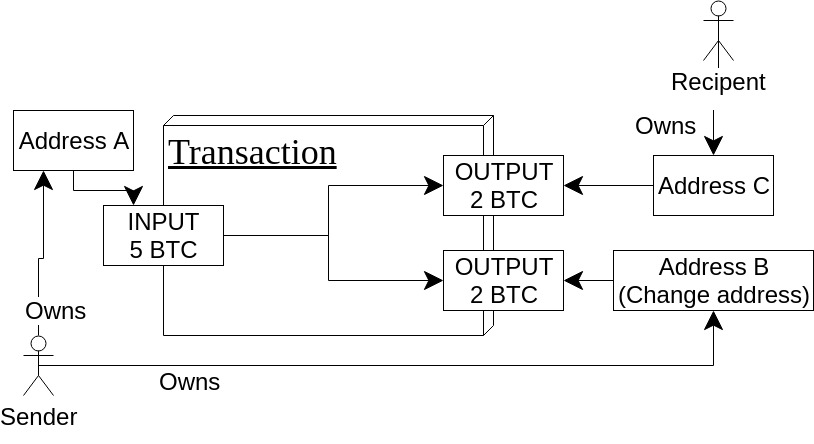
\includegraphics[width=1\textwidth]{change}
    \caption{Mechanism of change address}
    \label{change}
\end{figure}
 
When sending bitcoins from bitcoin wallet,
 wallet software creates transaction data and signs it with required private keys.
 Then it sends it to one or multiple bitcoin nodes.
Nodes collect transactions from users and broadcast them to other nodes on best effort basis.
The validity of the transaction is later checked by miners and added to the newly generated block
in blockchain.

\subsection{Mining}

The purpose of miners is to verify transactions and protect blockchain
from being overwritten by malicious third party.
Miners are running bitcoin nodes and mining software,
which enables them to create a new block of transactions,
add it to blockchain and broadcast a new, longer version, of blockchain to other nodes.
Finding a new block of transactions is a hard problem from computational perspective.
The SHA256 hash of newly generated block must be lower than given number called difficulty.
The lesser is the difficulty, the harder is it to find the new block.
Difficulty is adjusted every 2016 blocks in order to match the computanional power of miners,
so that new blocks are generated on average once per 10 minutes.

Each block must contain the hash of the previous block in the blockchain, so it is impossible
to precompute the problem for blocks that will come further in the future. 
Each block besides other things contain list of transactions and some free space,
where miners can insert random data to change the hash of the block.
Miners try to find block that satisfy SHA256 requirement
by brute-force by filling this space and when they find a solution,
they are able to generate a new block of transactions and broadcast it to other miners.
When miner generates a new block, he can claim all of the fees of transactions included in that block,
also he is able to create a special transaction called coinbase transaction that sends bitcoins from
nowhere to his address. By these coinbase transactions, new bitcoins are emitted into the network.
Blocks are limited by size and therefore may contain limited number of transactions.
It is possible for new transactions to be waiting for being added to the blockchain for some time,
because miners prefer to add transaction with higher fees to the next block.

\subsection{Tumblers}
Anyone can download blockchain and therefore obtain information about all bitcoin transactions that ever happened.
It might seem that bitcoin transactions are anonymous, but when the user sends bitcoins to
someone(exchange) who knows their identity, the recipient can pair the bitcoin address
the bitcoins came from to the identity of the sender.
Although bitcoin users usually use multiple bitcoin addresses,
their transactions and addresses are still 
susceptible to some analysis of blockchain transaction graph.
This might identify other addresses belonging to the owner of the address we already know.

Bitcoin Tumblers exist in order to prevent or at least obstruct such analysis.
A user sends bitcoins to the tumbler service and the service mixes his bitcoins
with bitcoins of other users by performing multiple transactions
between its bitcoin addresses. \parencite{moser2013inquiry}
  
The structure of these transactions differs for different tumbler services.
The user sends their bitcoins to an address owned by the tumbler,
then he generates a new, never used bitcoin address.
He than receives bitcoins from tumbler service to his new bitcoin address.

There also exist peer-to-peer tumblers(CoinJoin, SharedCoin, Coinswap),
that enable multiple users to directly create transactions to mix bitcoins among themselves.
These transactions can be performed multiple times with different actors.

\section{Tor - the onion routing}

Communication between browser and web server is usually done via HTTPS protocol.
This protocol uses asymmetric cryptography. The web server and browser exchange their public keys at the start of communication
and encrypt the data using these keys. Decrypting the data is possible only by corresponding private keys,
which the browser and web server keep locally. This protocol is susceptible to man in the middle attacks.
If the attacker has control over the transmission from the start of communication, he can place himself in the middle of communication and act as a web server for the user and as a user for the web server. To prevent these types of attack,
 a certification authority is needed. The certification authority is an institution that signs public keys, belonging to the web server.
 When the browser receives the public key, it automatically checks, if it is signed by any authority from its list of authorities and if not,
 it displays a warning or error message.
The HTTPS protocol encrypts data, but doesn't hide the identity of the user from the web server,
 and also the Internet provider can see, where is the user connecting. Tor aims to solve these issues.
 
Tor \parencite{dingledine2004tor} is a free open source software that provides access to Tor network. Tor network is a network of Tor nodes.
The goal of Tor project is to provide its users encrypted access to the Internet in order to prevent third parties
from eavesdropping and analysis of the transmitted data.
The usage of Tor can be detected by the third party, but the third party can not decrypt user's data that are transmitted
 via Tor. Some websites restrict access from Tor networks due to many risks involved.
Tor hides user's identity from the web server. Also Internet provider can just detect that user is connecting to Tor
, but can not identify the other side of communication and content of the transmitted data.

The simplest way for user to use Tor network is to install Tor browser bundle, which consists of
modified firefox browser and onion proxy. Onion proxy routes all traffic through Tor network.
Tor network consists of more than 6000 publicly available TOR nodes(also called relays or routers).
Anyone can run a Tor node, but there exist a subset of speciallized servers called directory authorities,
Directory authorities monitor relays and distribute a list of relays that are working and 
not under the same IP address.
Tor nodes splits into 3 groups, guard nodes, relay nodes and exit nodes.
A client achieves anonymous communication by proxying his traffic through
a chain of 3 Tor nodes, so called circuit, as it can be seen on picture \ref{tor}.
Client obtains public keys of these 3 Tor nodes from directory authority and negotiate
symmetric keys for encrypting the data with each node.
When client wants to send some data, he split them into fixed size chunks
called Tor cells and encrypt them with multiple layers of encryption by the symetric keys negotiated in previous step.
The schema of the encrypted Tor cell is on picture \ref{tor-packet}
Each node in the circuit decrypts the Tor cell and therefore removes one layer from it.
The exit node decrypts the last layer of encryption, reads the original data of the client and 
sends the packet to destination address. The reponse is than again encrypted by symetric keys
and sent back by the same circuit.
This way, each node only knows it's neighbours in the tor circuit, but doesn't know the rest of the circuit.
Tor employs multiple additional features for Tor relay selection and circuit building to prevent attacks
by behaviour and statistical analysis.
 
\begin{figure}[!htb]
    \centering
    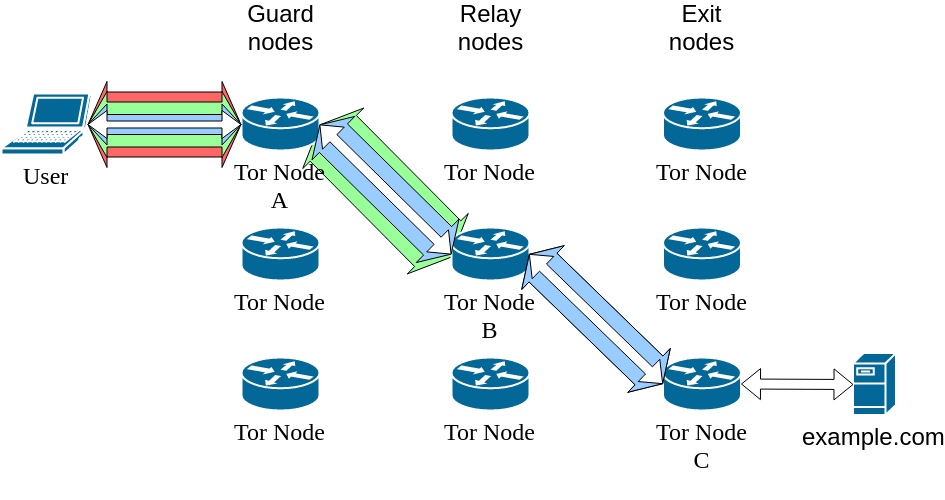
\includegraphics[width=1\textwidth]{tor}
    \caption{Tor routing schema}
    \label{tor}
\end{figure}
 
\begin{figure}[!htb]
    \centering
    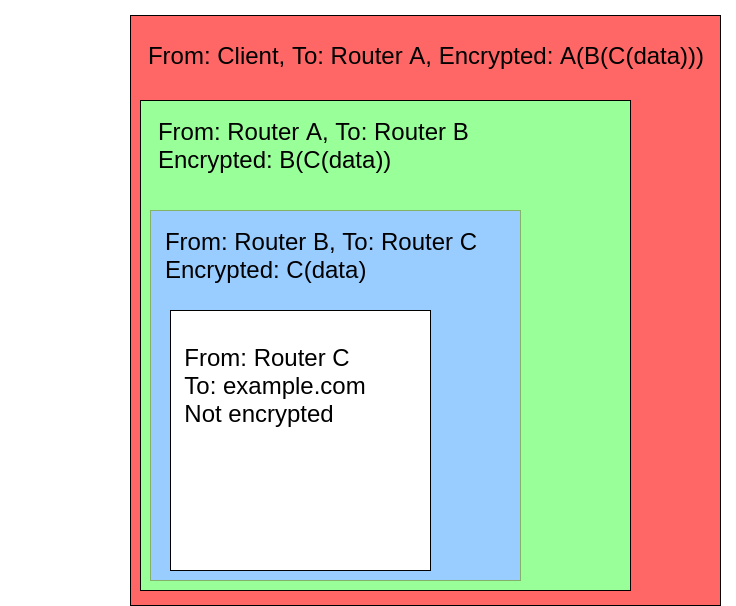
\includegraphics[width=1\textwidth]{tor-packet}
    \caption{Tor packed encryption schem}
    \label{Tor packed encryption schema}
\end{figure}
 
Cryptomarkets are running as a hidden services on TOR network.
Tor hidden services is a feature of Tor for providing a service (e.q. a webserver, IRC server etc.) over Tor network
without disclosing the server's IP address. The hidden services have special top level domain .onion.

When administrator of service wants to be accessed, he crates a RSA keypair.
The public key in base-32 encoding is identifier of service and service can be accessed by accessing URL identifier.onion.
The administrator choose some Tor nodes as introduction points and estabilish a circuit to each on of them.
The administrator than upload a descriptor of the service to 6 different hidden service directories(HSDir).
HSDir is a Tor node with a special flag that was assigned to it by TOR authorities.
The selection of HSDirs changes every 24 hours and can be deterministically computed from time and hidden service public key.
The descriptor contains the hidden service public key and signed list of introduction points.

When client starts connecting to the hidden service, he uses service's domain name(= public key)
to compute HSDirs with service descriptor. It download a service descriptor from HSDir with list
of introduction points. Client also generates one time secret, pick a random Tor node, asks
it to act as randevouz point and tell it the one time secret. 
Then client sends to introduction point a message for the service(encrypted by service's public key)
with the information about randevouz point and one time secret. The service recieves the message, connects 
to randevouz point and uses one time secret to match with client.
Randevouz point than just relays messages between client and hidden service.
All the connections mentioned above can be seen on picture \ref{onion service}.
Note that there is no direct connection between two servers during hidden service set-up,
all communication between servers are routed through regular Tor circuits.
Randevouz point just act as a relay between two Tor circuits.

\section{PGP}

PGP \parencite{Zimmermann:1995:OPU:202735} is a program for encrypting data
and communication between two parties using public key cryptography.
PGP is used for signing, encrypting and decrypting messages, mostly e-mails.
PGP was developed in 1991 as an open source, with the intention 
to provide an open, widely used standard for encrypted communication.
Nowadays, PGP program is not an open source anymore, but the standard is used by open source GPG software.

PGP uses public key cryptography. Unlike symmetric cryptography, public key cryptography
uses two different keys for encrypting and decrypting.
A user generates a pair of keys, a public key for encrypting emails sent to him and a private key, which the user
 keeps for himself and uses for decrypting messages encrypted with the associated public key.
 The user also publishes his public key, so other users can send him encrypted messages.

PGP is used in the context of online drug markets as a means of secure communication between vendors and customers.
Both vendor and customer have their public keys published on their profile page and use the public key of the other
party to encrypt messages to them. This enables vendors and sellers to keep their communication private also from the administrators of the marketplace.

\chapter{Related work}
\section{Blockchain analysis and de-anonymization of bitcoin addresses}

Multiple papers and tools were published regarding the analysis of blockchain.
Blockchain contains all bitcoin transactions and anyone can simply check
the source and destination addresses of every transaction in the system.
It is heavily encouraged for users of blockchain to use multiple bitcoin addresses
 and every major bitcoin wallet (software, for receiving and sending bitcoins) do so.
 It is therefore useful to detect addresses belonging to the same user.
 
The authors of first research article \parencite{reid2013analysis}
 parsed blockchain files to create a graph of bitcoin transactions, with vertices as transactions
 and edges between them represented bitcoins flowing from one transaction to another.
 They created so-called user graph by clustering addresses belonging to the same user.
 They used simple heuristics that the owner of all input addresses used in a transaction must be the same. The first version of this article  
was published in 2011 and dealt with a much smaller number of people using bitcoin and smaller transaction graph.
Their analysis also focuses on deanonymization through multiple aspects of bitcoin protocol,
while this thesis focuses on deanonymization from transaction graph and public data.

Androulaky \parencite{androulaki2013evaluating} performed clustering using two heuristics.
The first one is the same as \parencite{reid2013analysis} did that all inputs of transaction
belong to the same user. The second heuristics is clustering some outputs of the transaction with its inputs.
Most transactions have two outputs, one is owned by the transaction recipient,
the other one is called change output and is owned by
the sender. The mechanism of change output is described in chapter \ref{btcadd} and the heuristics in
chapter \ref{Using own transactions to identify market wallets}.
If the transaction has two output addresses A and B, A has appeared in blockchaih
before and B not, than he assumes that B is the change address, because it is common
for wallet software to generate new never used addresses for change outputs.
They also employed multiple clustering techniques based on the behaviour of users.
 They tested the success of their clustering techniques in their simulated bitcoin 
 environment.

Advanced and similar work was done by \parencite{spagnuolo2014bitiodine}. They downloaded the blockchain, transformed to
 the database
and performed clustering to get a graph of transactions between users.
Then they developed a tool, which scraped data from multiple locations(Bitcointalk and bitcoin-OTC forum) to link off-ch
ain data and identities to bitcoin addresses.
They tested the tool on few popular transactions related to the seizure of Silkroad marketplace.

Similar work to this thesis was done by \parencite{fleder2015bitcoin}.
This paper use data from Bitcointalk, the most popular bitcoin forum. 
They apply a simple algorithm to group multiple bitcoin addresses belonging to one user together.
Then they use the scraped data to show
that some of the Bitcointalk users were using Silkroad marketplace or other popular services accepting bitcoin.
 
Ron and Shamir \parencite{ron2013quantitative} focus on bringing
interesting statistics about bitcoin transaction graph
and provided a detailed analysis of really big bitcoin movements ( more than 5000 BTC) 
through transactions in the network.
In their other study \parencite{ron2014did}, they analyzed transactions performed by Ross Ulbricht,
who was the administrator of Silkroad marketplace.
The FBI published their bitcoin address, which they used to collect all seized bitcoins from Ross Ulbricht.
They took the size and frequency of transactions related to the seized bitcoins prior to the seizure and compared it to the estimated income of Silkroad. They found discrepancies between the
relatively stable income of Silkroad marketplace and unstable balances in bitcoin addresses
that were seized by FBI. They conclude that FBI seized around 22\% of Ross Ulbrich bitcoins
and found addresses that posses a some of these bitcoins, which has not been used since Ross' arrest.

In contrast to previously mentioned papers, Meiklejohn \parencite{meiklejohn2013fistful} 
doesn't only passively scan blockchain, they actively send bitcoins to addresses of
well-known services to track their bitcoins in the following transactions executed by the service.
They also used the same two heuristics for clustering addresses
as Androulaki. \parencite{androulaki2013evaluating}
They concluded that the network does not offer enough anonymity and large transactions can be traced.

All of the previously mentioned works had to deal with much smaller transaction graph,
as the usage of bitcoin grew significantly over the last year. 
To the best of my knowledge,
no previous work utilizes so many resources of data as this work.
Also, the aim of our tool is to be able to detect, if some specific bitcoin address of 
investigator's interest was somehow connected to Valhalla drug market, or at least find nearby
deanonymized addresses in the transaction graph to help with further investigation.

\section{Behaviour of drug markets users and operators}

Emerging cryptomarkets brought the attention of the scientific community
and lots of articles have been published related to the phenomena of drug trafficking via the Internet.
Most of these papers were investigating the topic from the social
and criminology perspective and performing qualitative analysis.
\parencite{aldridge2014not}
\parencite{barratt2014use}
\parencite{christin2013traveling}
\parencite{dolliver2015criminogenic}
\parencite{van2013silk}
\parencite{walsh2011drugs}
\parencite{martin2014lost}

There are only a few articles focusing on statistically describing fully operating drug market and it's vendors
by collecting and analyzing data from a cryptomarket webpage. Short description of works like that follows.
Aldridge \parencite{aldridge2017delivery} scraped Silkroad in September 2013, the most popular cryptomarket of that time
.
He focuses on how the vendors and buyers perceive a risk of arrest and attempt to limit them.
He concludes that users of cryptomarket are aware of the risks both related to their physical and online activity
and actively reduce their risk.

Decary \parencite{decary2017repeat} focus on answering the question, how loyal are buyers on cryptomarkets to vendors. It seems, those popular vendors successfully build their loyal
customer base. These findings make sense, given the natural health risks related to using drugs,
customers prefer vendors with high reputation and trust.

Broseus \parencite{broseus2016studying} restricted his research to vendors shipping from Canada
and track their activity through multiple markets. His findings include that same vendors
use same usernames and sometimes PGP keys on multiple marketplaces because reputation
is highly valued in these cryptomarkets and so vendors try to keep it when moving to the new marketplace.
Also by his findings, some vendors are highly specialized in selling on the category of drugs, while others offer a wide range of drugs.

Article by Doliver \parencite{dolliver2016characteristics} is most similar to this work.
They scraped and analyzed two popular cryptomarkets, Agora and Evolution and quantitatively assess
the characteristics of vendors from both markets, focusing on the difference
 between different markets' vendor populations.

 All previously mentioned works were analyzing cryptomarkets that are not operational nowadays,
 while this work focus on describing the vendors from currently operating drug market Valhalla 
 and examine, if the behaviour of vendors or the nature of cryptomarkets
 has changed significantly. We also not only passively scraped cryptomarket's webpage,
 but also created a user account on the marketplace and sent/received bitcoins from the marketplace
 in order to get data about the cryptomarket's flow of money.
 
\chapter{Methods and tools of data retrieval and analysis}

\section{Valhalla cryptomarket webscraping}
\label{Valhalla cryptomarket webscraping}
We scraped data from Valhalla cryptomarket
during january and february 2018. 
We used official Tor daemon and software called privoxy, to create a local proxy that will redirect all
incoming traffic through Tor network. The privoxy was needed because Tor daemon creates SOCKS proxy,
which can not be used by wget. So we created an HTTP proxy by privoxy,
which redirected the traffic through Tor SOCKS proxy.
we did not have to implement any login and captcha solving functionality
for web scraping Valhalla market, because all the webpages about market
listings, vendors and feedbacks are available without logging in.

Addresses of all market listings are in pattern\newline
\texttt{http://Valhallaxmn3fydu.onion/products/\textbf{xxx}} where \texttt{\textbf{xxx}}
is a number incrementing with each new listing.
The last listing had number 103770 and only 25309 numbers lead to the valid listing page.
Rest of the numbers lead to 404 error. We believe,
that these numbers refer to listings that were delisted by the vendor or administrator.


We wrote a small script in bash to iterate through all of the listings
and download them using wget command line tool.
After downloading all the listing pages,
we parsed the downloaded files using python and common Linux command line tools(cat, grep, cut, sed).
We were not using python HTML parsing libraries(like beautifulsoup) for parsing downloaded
webpages because HTML elements of Valhalla web pages don't have any unique identifiers
and so these libraries bring us no advantage.
 
By scraping the listings pages, we got unique vendor nicknames,
which we used for downloading and scraping vendor's profile and feedback pages.
The shortcoming of this method is, that we were able to download and analyze only sellers, 
that have at least one active listing at the time of data collection. 
Vendor profile pages were in format \texttt{http://Valhallaxmn3fydu.onion/\textbf{xxx}}
and their reviews in the format
 \texttt{http://Valhallaxmn3fydu.onion/\textbf{xxx}/palautteet} where \texttt{\textbf{xxx}}
is a vendor nickname. 
 
From each listing, we parsed:

\begin{table}
    \caption{Data scraped from listings}
    \label{datalist}
    \begin{tabular}{|l|l|}
 Variable & data type\\
 Vendor's nickname & string\\
 Subcategories & 3 strings\\
 Title of listing & string\\
 Price & float\\
    \end{tabular}
\end{table}

From each vendor, we parsed:

\begin{table}
    \caption{Data scraped from vendor pages}
    \label{datavendor}
    \begin{tabular}{|l|l|}
 Variable & data type\\
Vendor's nickname & string\\
positive and negative feedbacks & 2 integers\\
revenue & integer 0<=x<=10000USD\\
PGP key & string, is not mandatory for all vendors\\
Country & string, country from which vendor ships if available\\
    \end{tabular}
\end{table}

From feedback page, we parsed the following variables for each feedback:
\begin{table}
    \caption{Data scraped from feedback pages}
    \label{datafeedback}
    \begin{tabular}{|l|l|}
 Variable & data type\\
vendor nickname & string\\
rating & 1-5\\
date & Timestamp, days resolution\\
buyers nickname & string of length 4\\
money the buyer spent & int\\
trades the buyer did & int\\
   
    \end{tabular}
\end{table}

\section{Valhalla cryptomarket metadata scraping and analysis}

We thought that metadata from the photos of drugs, which vendors upload
to show in their listing, might contain some information leading to identity disclosure.
We downloaded 20 images from valhalla market and examined 
EXIF metadata using \texttt{identify} command line tool.

Only metadata directly depending on image content, like the amount of red, green and blue colours
were different for different images.
Metadata that could potentionally help dislosing user identity,
like date of creation nad modification, signature and name of software version were the same for all images.
The software version contained exactly this string:
"ImageMagick 6.8.9\-9 Q16 x86\_64 2017\-07\-31 http://www.imagemagick.org"
ImageMagick is popular software library used for manipulating images, so it seems
that market automatically rewrite EXIF metadata in uploaded images in order to protect privacy of users.
To test this hypothesis, we created vendor account and uploaded an image with
custom-made EXIF metadata. We than downloaded the uploaded image from webpage and 
saw that EXIF metadata were indeed overwritten.

We tested if every transaction that is happening on drug market has its counter transaction
in bitcoin blockchain.
We deposited some BTC to cryptomarket and bought a licit virtually deliverable
product(Guide on weightlifting) and checked if anything happened to the deposited bitcoins.
There was no follow up transaction happening for weeks after the deposit transaction was done.
This means that markets don't transfer bitcoins when service or goods are bought.
All of bitcoin transactions that these drug markets do 
are accepting bitcoins deposits,
sending bitcoins to withdrawing users and possibly bitcoin tumbler transactions, it they
use such service.
We made multiple deposits and withdrawals from Valhalla in order to track,
where were the deposited bitcoins later transfered and where have the withdrawn
bitcoins came from. These deposits and withdrawals have been
used in our application for clustering bitcoin addresses owned by Valhalla cryptomarket.

We tried to scan ports of drug markets servers and fingerprint their web server,
in order to find any vectors for further information gathering. 
We scanned Valhalla server using netcat and found that the only opened ports are 80(redirect to https) and 443(HTTPS),
which is used by web server. The webserver was popular software called nginx, as we detected
both from HTTP headers and from webserver fingerprinting tool httprecon.
The result of port scan and web server fingerprinting doesn't indicate
any new vectors for gathering data about cryptomarket.

Some vendors have published their PGP keys on their profile page.
We scraped 150 PGP keys and tested them ROCA vulnerability via python module roca-detect. None of these keys were vulnerable.
All these PGP keys were searched for User-Id in metadata and found user-Ids were seached by google.
None of the searches for user-Ids(both nicknames and mail addresses) returned usable results.
Some of the usernames were just briefly mentioned in some posts on anonymous forums like 4chan.org.

\section{Publicly available data scraping}
\label{Publicly available data scraping}

In order to have some bitcoin addresses and bitcoins linked to identities,
we searched Internet for pages, where are bitcoin addresses tied to offline or virtual identities.
The sites that we have decided to scrape were Bitcointalk forum, Reddit,
Twitter and bitcoin.info.
The Bitcointalk is the most popular Internet forums
related to cryptocurrencies. URL address of profile page on Bitcointalk
and contains the profile number, which starts at 1 and is incremented by 1
for each new profile. It is therefore easy to iterate over all forum's profiles,
including the ones with no posts, and check if they have associated bitcoin address.
The scripts bitcointalk-scraper.py visit profile pages of all profiles on the forum and scrape usernames and bitcoin addresses. 
The Reddit and Twitter were scraped by twitter-scraper.py and reddit-scraper.py
The script contain several hardcoded phrases like "Donate bitcoin" and "bitcoind address" and scrapes 
result of searches for such phrases.
Bitcoin.info is a webpage that serves primarly as bitcoin blockchain explorer. Secondary,
it gathers multiple statistics about bitcoin blockchain and also offers
third parties having their bitcoin address and identity listed on their webpage.
The generated identities are stored as rows in csv files that have 3 collumns:

\begin{enumerate}
 \item bitcoin addres
 \item URL where was the address scraped
 \item nickname of the associated identity
\end{enumerate}

\section{Using own transactions to identify market wallets}
\label{Using own transactions to identify market wallets}

Valhalla cryptomarket generates unique deposit address for each new user.
When user wants to buy something, he needs to deposit bitcoins to deposit address,
that will top up his account balance and he than uses this account balance to buy stuff.
Vendor or user can request withdrawing their bitcoins from cryptomarket and so
the cryptomarket decrease their account balance and sends bitcoin to user's address.

For identifying bitcoin addresses that are owned by Valhalla cryptomarket, we 
deposited small amount of Bitcoins to our user accounts on Valhalla cryptomarket and
performed multiple withdraws by smaller amount than the deposited on to recieve bitcoins back.
When we requested bitcoin withdrawals, we recieved bitcoins from different addresses
than the deposit one. We consider the deposit address and all addresses we recieved
bitcoins from during withdrawals as owned by cryptomarket.

Knowing just about these addresses would no help us decide
if someone sent or recieved bitcoins from Valhalla cryptomarket.
It is common for any service accepting bitcoins to
use multiple bitcoin addresses, because it's common practice and even default behaviour for
bitcoin core and other bitcoin wallet software. Unique deposit address for each
account on Valhalla market is required for each user, so that system can associate
bitcoin transaction with Valhalla market account.
In order to solve this issue, we used two heuristics that were widely used
in previous works \parencite{androulaki2013evaluating}\parencite{reid2013analysis}
for clustering bitcoin addresses belonging to same user.

The first heuristics simply states that all inputs of one transaction belong to same user. This is logical,
since users generally don't share their private keys and collaborate on creating one transaction.
When transaction have multiple inputs with different bitcoin addresses, we assume that all of these addresses are owned by
one identity.

The second heuristics focus on detecting change address described in chapter \label{btcadd}.
The goal of second heuristics is to detect change addresses in the transactions.
When one transaction has two outputs with two different addresses, we assume, that one of them is change
address and is owned by the sender.
We than search through the the blockchain for the first occurence of each address of the outputs of the 
transaction. If one of the output addresses had been used before the transaction and second not,
than we can safely assume, that the second one is change address\parencite{androulaki2013evaluating}.

Both of these heuristics are pretty strict and have just a negligible chance of falsely merging
addresses not belonging to the same user\parencite{androulaki2013evaluating}.
There exist multisignature wallets and also few proposals for anonymization methods that could make
these heuristics missleading(like CoinJoin mixer and dark wallet) 
, but these contribute to negligible percentage of transactions.

We measured the success of heuristic clustering in two ways.
We had two accounts on Valhalla market, each performing 1 deposit of 0.011 BTC and immidiatelly 10 withdrawals of
0.01 BTC, with roughly 0.001 BTC spent on cryptomarket fees.
For the first account, we performed these transactions on 8.2.2018, the second one on 4.3.2018.

We created new bitcoin wallet via mycelium mobile app, deposited bitcoins to it
from bittrex exchange and used that wallet only with first account.
The second bitcoin wallet was used only by second account and created by coinomi mobile app. 
Bitcoins were deposited to it from coinmate.cz bitcoin exchange.
We installed both these wallets and generated new, never used bitcoin address in each one, and also
recieved bitcoins from two different exchanges in order to not affect
our measurement with the fact, that we are owners of both bitcoin addresses.

We than ran our application and looked into the neo4j database, that stored
blockchain transaction graph and associated identities.
We checked the cryptomarket's address we identified by our deposits and withdrawals,
if they were clustered as one identity. The table \ref{clustertest} shows, how many identities
were associated with given deposits and withdrawals.

We checked, how much bitcoins have these
identities recieved between 15.1 and 15.2. We scraped Valhalla cryptomarket between 14.2 and 15.2
and we got data from feedback pages, which we used to estimate 
the minimal amount of bitcoins users spent over the previous month on Valhalla market.
We estimated in chapter \ref{stats}, that users spent at least 527730EUR during that one month time.
With average bitcoin price 8219EUR it roughly equals 527730/8219 = 64.2BTC
The amount of bitcions these identities recieved is also in table \ref{clustertest}.

\begin{table}
    \label{clustertest}
    \begin{tabular}{|l|l|l|l|}
    Identity &\multicolumn{1}{|p{4cm}|}{\centering Deposits:withdrawals \\ from first account }&\multicolumn{1}{|p{4cm}|}{\centering Deposits:withdrawals \\ from second account}
    & \multicolumn{1}{|p{2cm}|}{\centering recieved \\ bitcoins }\\ 
    1&   1:0 & 0:0 & 0.011  \\ 
    2&   0:0 & 1:0 & 0.011  \\ 
    3&   0:4 & 0:1 & 3.15  \\ 
    4&   0:2 & 0:0 & 0.7  \\ 
    5&   0:1 & 0:1 & 1.5  \\ 
    6&   0:1 & 0:0 & 0.15  \\ 
    7&   0:1 & 0:0 & 0.1  \\ 
    8&   0:1 & 0:0 & 0.1  \\ 
    9&   0:0 & 0:3 & 1.23  \\ 
    10&  0:0 & 0:2 & 0.12  \\ 
    10&  0:0 & 0:2 & 0.37  \\ 
    11&  0:0 & 0:1 & 1.1  \\ 
    \end{tabular}
    \caption{Mapping of found identities to addresses used in deposits and withdrawals
    each row in table represent one identity and numbers indicate how many deposits/withdrawals from
    our accounts were associated with that identity}
\end{table}

Our heuristics were not enough to cluster majority of market's transactions/addresses as one identity.
Hovewer, with just two accounts, 2 deposits and 20 withdrawals, we were able to identify 8.52BTC out of estimated
64.2 BTC the market recieved during that one month timeframe.

\chapter{Application for searching nearby identified addresses}

This chapter describes our application for searching in gathered data.
The application architecture is depicted in figure \ref{application_architecture}.
It consists of multiple python scripts that falls into 5 categories.

\begin{itemize}
 \item Scripts for scraping Valhalla market
 \item Scripts that parse bitcoin blockchain and also scrape data from publicly available sites mentioned in section \ref{Publicly available data scraping}.
 \item The script which imports data to the database, creates indexes and runs heuristics mentioned in chapter \ref{Using own transactions to identify market wallets}.
 \item Webserver that handles GUI requests and retrieves data from database.
 \item The web GUI written in HTML/JS/CSS for sending requests to webserver and visualisation and search in retrieved data. 
\end{itemize}


\begin{figure}[!htb]
    \centering
    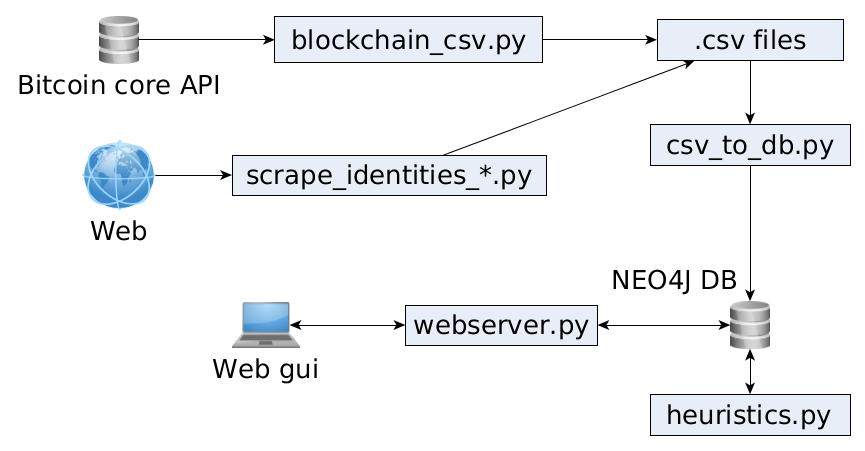
\includegraphics[width=1\textwidth]{application_architecture}
    \caption{Architecture of application}
    \label{application_architecture}
\end{figure}

Scripts for scraping Valhalla market in order to get statistical data used in next chapter are in statistics folder.
Script listing-scraper.sh goes through Valhalla listings and download the HTML source code of these pages.
Script listing-parser.py process the downloaded pages and generate listings.csv file with informations about listings.
Seller-scraper.py opens listings.csv and for download HTML source of vendors' profile pages. 
Seller-parser.py proccess downloader vendor's profile pages and generates sellers.csv and feedbacks.csv.
The variables and data types stored in these .csv files are described in chapter \label{Valhalla cryptomarket webscraping}.
in tables \ref{datalist}, \ref{datavendor} and \ref{datafeedback}. We used these generated .csv files for
bringing statistics about Valhalla cryptomarket in the next chapter.

The scripts for obtaining data the application needs are in folder identity--scraping.
Each of scripts named scraper\_{bitcointalk,blockchaininfo,reddit,twitter}.py scrape webpage mentioned
in it's name and generates a .csv file with 3 collumns: bitcoin addres ,URL where was the address scraped
and associated identity( e.q. nickname). These files with identities are later imported into neo4j database.
Script blockchain\_to\_csv.py uses bitcoin-core api to iterate through blockchain transactions
and generate several csv files with the data from blockchain that are needed by application.
The script generates multiple csv files, that will be later imported to neo4j database.

In order to create a tool that will effectively search and visualize blockchain data and the 
data we scraped, we need to store the blockchain and identity data locally in that way, so that common
graph algorithms, heuristics and searching can be effectively performed.
The natural representation of transactions happening between
bitcoin addresses is a graph, so we decided to import all the data into Neo4j graph database. It's the
most widely used graph database with native support for common graph algorithms.
Simple representation with addresses as nodes and transactions between them as edges in not
sufficient for our case, because we need to represent
outputs, inputs and time of transactions in the database in order to be able to compute previously mentioned heuristics. 
The graph schema is in figure \ref{neo4jschema}. The entities in the schema are represented as vertices
 in the database and relationships between them are edges.

The importing script ($csv\_to\_neo4j.py$) is responsible for parsing
previously generated .csv files and importing the data into neo4j database.
Having csv files as interminiary step between parsing blockchain and importing it to database
is useful for debugging application and also provides easy way to
use application with different blockchain or customly generated data.

\begin{figure}[!htb]
    \centering
    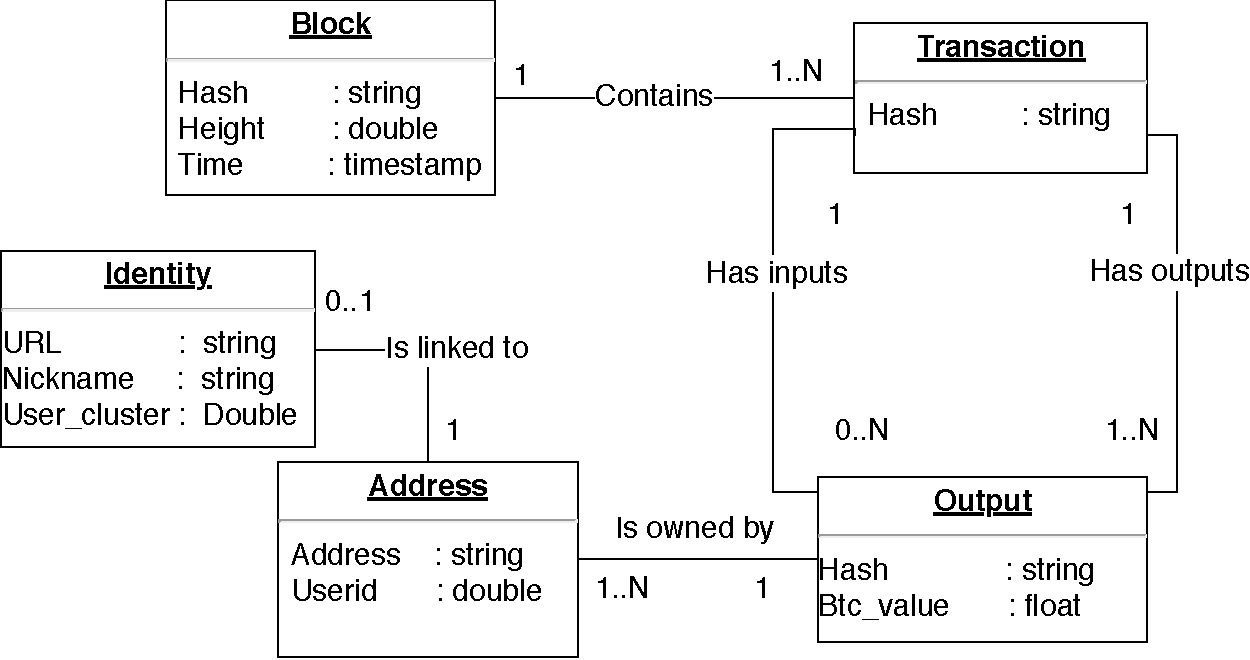
\includegraphics[width=1\textwidth]{neo4j-schema}
    \caption{Neo4j database ER diagram}
    \label{neo4jschema}
\end{figure}

Script cluster\_identities.py connects to database and run the heuristics from the chapter
\ref{Using own transactions to identify market wallets}.
It labels each address in our blockchain transaction graph
with unique ID representing unique identity. The outputs/inputs owned by the each address are labeled
with same ID. Script then alternatively runs first and second heuristic,
each time rewriting IDs of merged address(and it's outputs/inputs), so that 
addresses marked by the heuristic as belonging to the same identity have same user ID.
It stops, when there are no changes in IDs among addresses
(e.q = heuristics don't merge any addresses under one identity)
The webserver.py connects to local neo4j database with the schema and data generated by previous
scripts and starts local flask webserver that provides web gui on port 5000.

The GUI has one input form, where user should write the bitcoin address he is interested in.
The GUI than shows information about the inserted address, nearby addresses and found identities.
It consists of 3 parts shown in the screenshot \ref{guiscreen}.
The first part is simple HTML form where user submit bitcoin address he is interested in.
After submission, the rest of the parts show information about given address.
The table in part 2 show list of nearby addresses with known identity. The distance is number of transactions
between inserted address and addres in table. It also shows where the URL the identity was found
and amount of bitcoins that wen through that address over the history of blockchain.
In section 3, there are two pie charts. The first pie-chart shows bitcoins that were recieved by the address
and what percentage of recieved bitcoins was the application able to link to some identity.
The second pie chart show the same information for outgouing bitcoins, the percentage of bitcoins that were sent from this address
and ended up in address that we were able to find associated identity.

\begin{figure}[!htb]
\hspace*{-1cm}
    \centering
    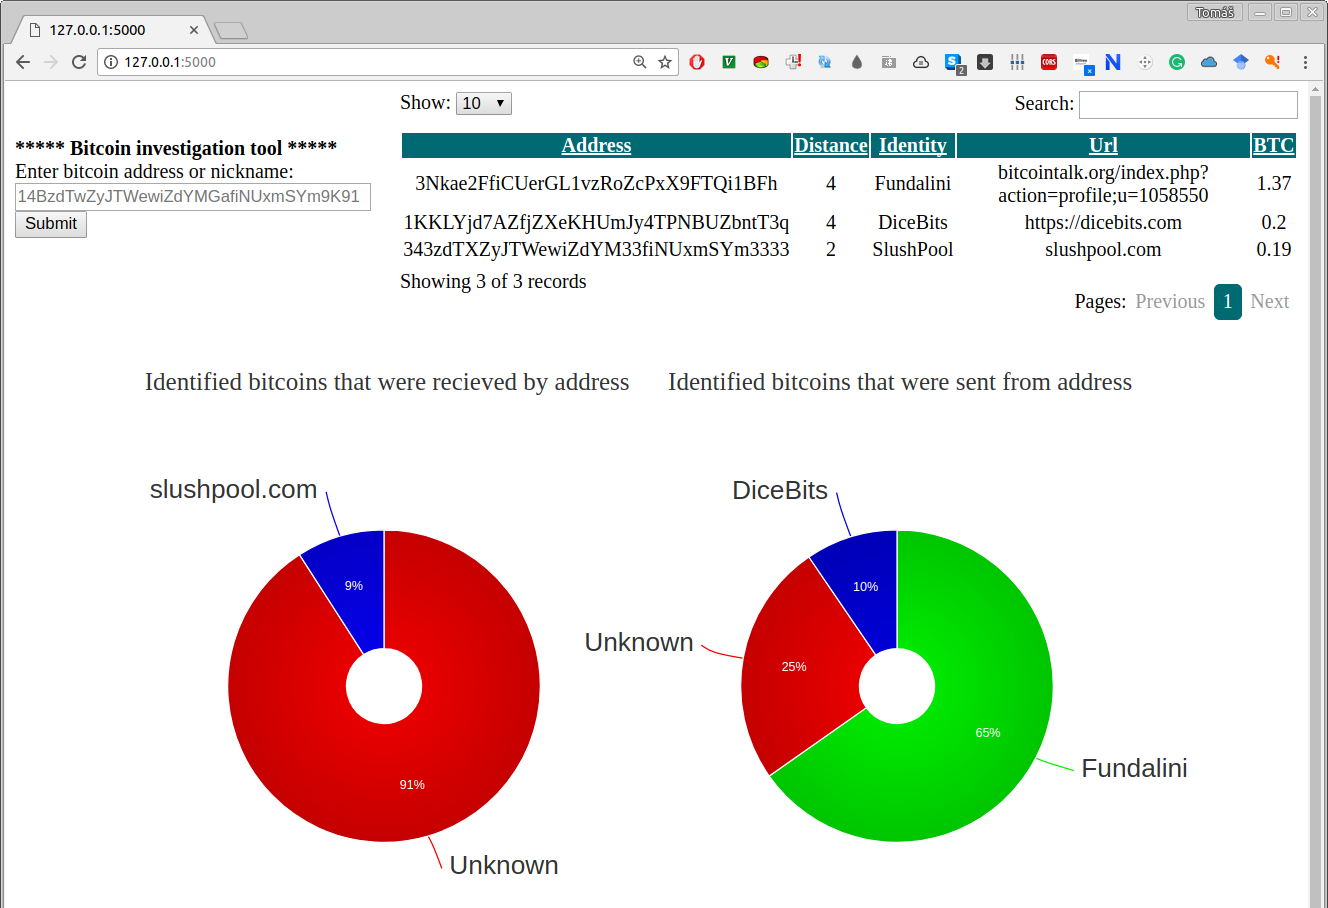
\includegraphics[width=1\textwidth]{shot}
    \caption{Screenshot of Gui}
    \label{guiscreen}
\end{figure}

\chapter{Statistics of Valhalla cryptomarket}
\label{stats}


We managed to scrape 25309 listings, 981 vendors and 6381 feedbacks.
There were 17314(68\%) listings related to selling drug substances, the rest
were related to ebooks, premium accounts, guns, fake IDs etc..
Vendors had from 1(90 vendors) to 1083(1 vendor)
active listings, with average of 25.69 (SD = 58.06)
and median = 11.00 listings per vendor.
Most vendors tend to have just few active listings,
as it can be seen on histogram \ref{listingsxsellers}.
The histogram does not show 19 vendors with more than 200 listings.

\begin{figure}[!htb]
    \centering
    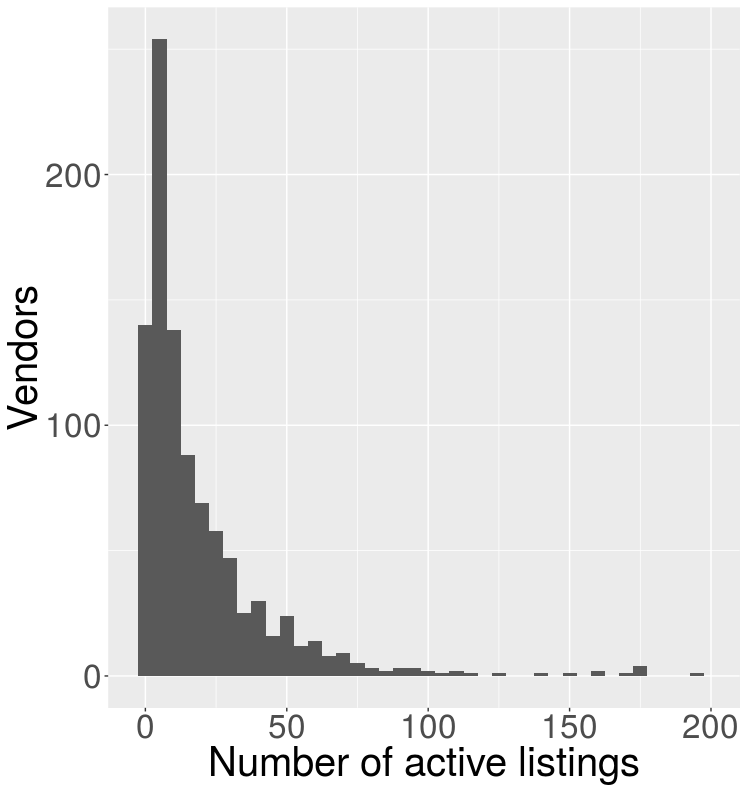
\includegraphics[scale=0.6]{listingsxsellers}
    \centering
    \caption{Histogram for number of active listings vendors have}
    \label{listingsxsellers}
\end{figure}

Vendors were shipping drugs from 39 distinct countries,
the frequency of countries the vendors were shipping from is in table \ref{shipcount}.
Table \ref{richvendors} list countries of vendors that have achieved 10000EUR(150 vendors \~ 15\% ) or more in revenue.
Valhalla was originally estabilished as a local Finnish crypto market.
That seems to be the reason for surprisingly many vendors shipping from Finland and also large percentage
of Finns among high revenue vendors, because they might be on the market since
the time it was not internationally popular and had more time to generate revenue.

\begin{table}
    \caption{Countries that vendors ship from}
    \label{shipcount}
    \begin{tabular}{|l|l|}
    Countries vendors are shipping from  & Count of vendors\\
        Finland                                      & 28  \\ 
        United Kingdom                               & 23  \\ 
        United States                                & 16  \\ 
        Germany                                      & 13  \\ 
        Netherlands                                  & 12  \\ 
        France                                       & 5   \\ 
        Norway                                       & 5   \\ 
        Spain                                        & 4   \\ 
        Canada                                       & 4   \\ 
        Australia                                    & 3   \\ 
        Poland                                       & 3  \\  
        Others                                       & 31   \\
        Unknown                                      & 834  \\
    \end{tabular}
\end{table}

\begin{table}
    \caption{Countries high revenue vendors ship from}
    \label{richvendors}
    \begin{tabular}{|l|l|}
    Country & Count of vendors\\
Finland & 24 \\
UK & 13 \\
USA & 10 \\
Germany & 6 \\
Netherlands & 6 \\
Norway & 4 \\
Others & 20 \\ 
Unknown & 69 \\
    \end{tabular}
\end{table}

\begin{figure}[!htb]

\subfloat{
    \centering
    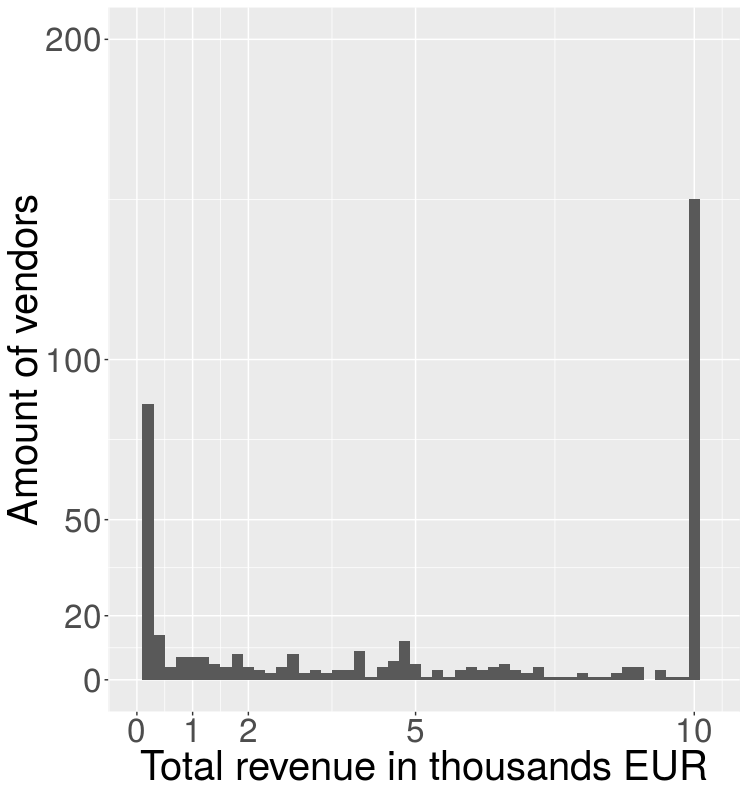
\includegraphics[width=0.5\linewidth]{total-rev}
%    \caption{Vendors by total revenue}
\label{total-rev}
}
\subfloat{
    \centering
    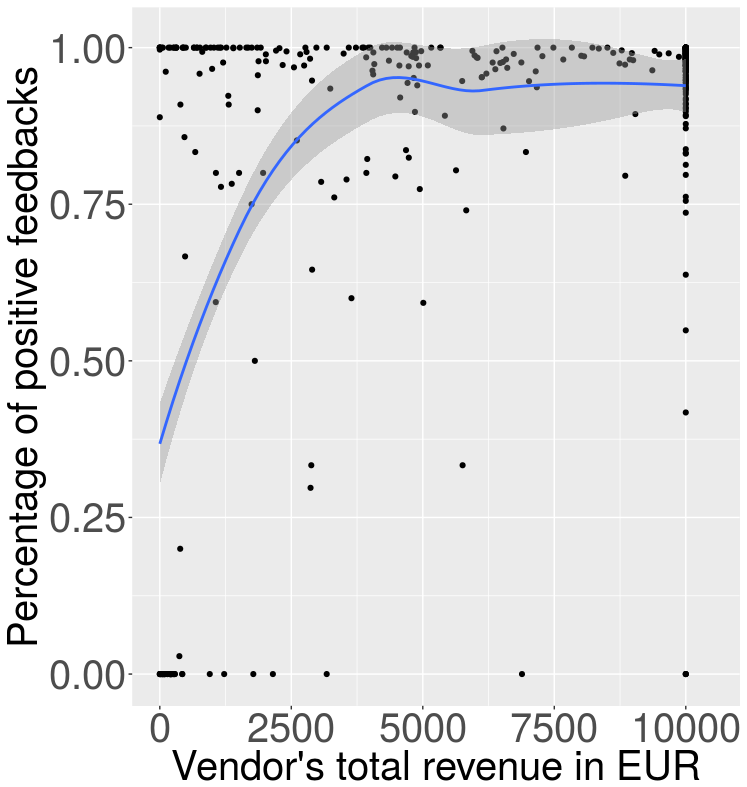
\includegraphics[width=0.5\linewidth]{posratrev}
\label{posratrev}
    %\caption{Vendors revenue related to ratio of positive feedbacks with linear regression}
    }
    
\caption{Distribution  of vendors by their revenue}
\end{figure}



We looked at total revenue of vendors, which is depicted in figure \ref{total-rev}. 
The total revenue mentioned in the vendor's profile page is capped at 10 000 Eur.
There are two major groups of venders regarded to their revenue. 
Majority(598 vendors \~ 60\%) of vendors have not had any positive or negative feedbacks and all of these vendors
but 3 earned less than 300EUR on cryptomarket over their lifetime.
Note, that we were able to scrape just the vendors with active listings,
so there might be much more vendors who stopped using Valhalla after
not being able to earn substantional amount of money.
The second group is 150 vendors (15\%) who earned 10 000 EUR or more.

Vendors who had high revenue maintained high ratio of positive feedbacks.
When counting only vendors with more than 10 reviews(304 vendors \~ 31\%),
the mean is 93.7\% and median 98.3\% of positive feedbacks.
Vendors with 1 to 10 reviews had on average 27.2\% of positive feedbacks.
Figure \ref{posratrev} shows the the distribution of vendors with similar
positive feedbacks ratio and revenue nad its LOESS curve.
These findings indicate, that market is competitive and
having bad reputation during first few sales shuts down any opportunity
for the vendor to continue selling his goods and that majority of vendors don't succeed or use
market sporadically.

The figure \ref{listingxprice} shows distribution of prices of all listings in
 the market on the left graph and on the right graph is the distribution of prices
 of listings linked in feedbacks. Some listings might be counted multiple times or not at all
 in the right graph, because one listing might be bought several times or not at all
 and therefore generate multiple or no feedbacks. We expect that distribution
 of prices in these feedbacks reflects more accuratelly the prices of the goods or services
 that are actually bought at market, because feedbacks can be given only by users who
 bought something from vendor. We calculated price of listings in EUR as 
 price in bitcoin multiplied by the average price of bitcoin for 30 days before the scraping
 (8219 EUR for 20.1.2018 - 20.2.2018, daily prices taken from blockchain.info).
 
 The average price of listing is 336.2 Eur(1368.2 SD!) with median of 71.3 Eur,
 while feedbacks had average 82.7Eur(150.7 SD) with median of 55 Eur.
  There were only 22(0.3\%) feedbacks with price > 1000EUR
 and only 5(0.01\%) feedbacks with price > 2000 Eur.
  There were 1533(6.05\%) active listings
 with price greater than 1000 EUR
 673(2.7\%) listings them with price greater than 2000 Eur.
 The price distributions in \ref{listingxprice} shows,
 that while there exist a lot of free or very expensive listings,
 majority(5937 93\%) of trades were between 0 and 200 EUR.
 There were 115 free listings on the market,
 but no one of them was mantioned in feedbacks.
 The free listings had titles like "CARDING SERVICE *FREE*",
 "Custom order", "Free Carding Tutorial 2017" and "FREE SAMPLE 84\% MDMA CRYSTAL ROCKS"
 The titles of expensive listings don't indicate that 
these listings are somehow special except the price.

\begin{figure}[!htb]
\label{listingxprice}
\subfloat{
\label{listingxprice}
    \centering
    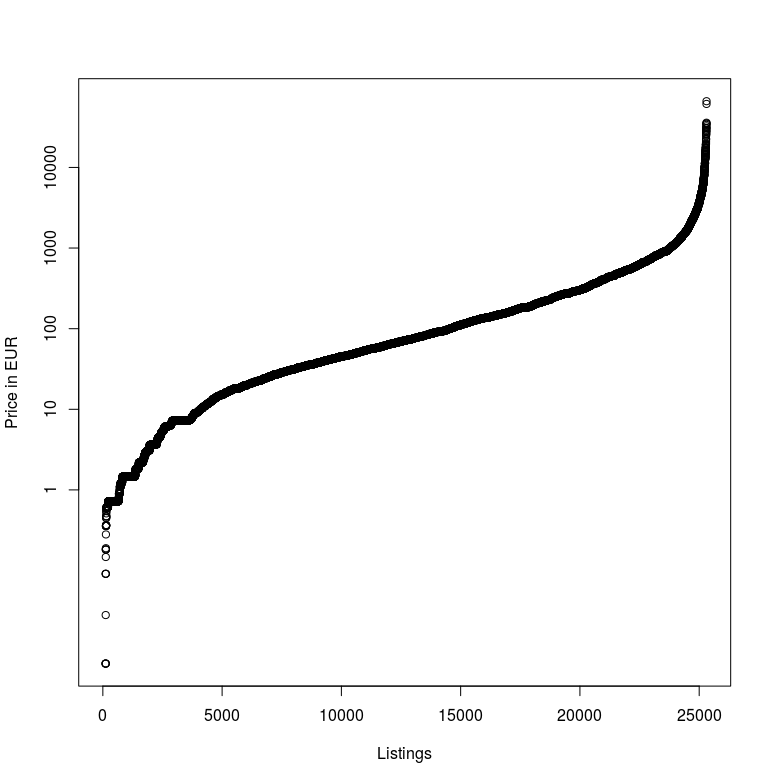
\includegraphics[width=0.5\linewidth]{listingxprice}
    %\caption{Prices of listings}
}
\subfloat{
\label{flistingxprice}
    \centering
    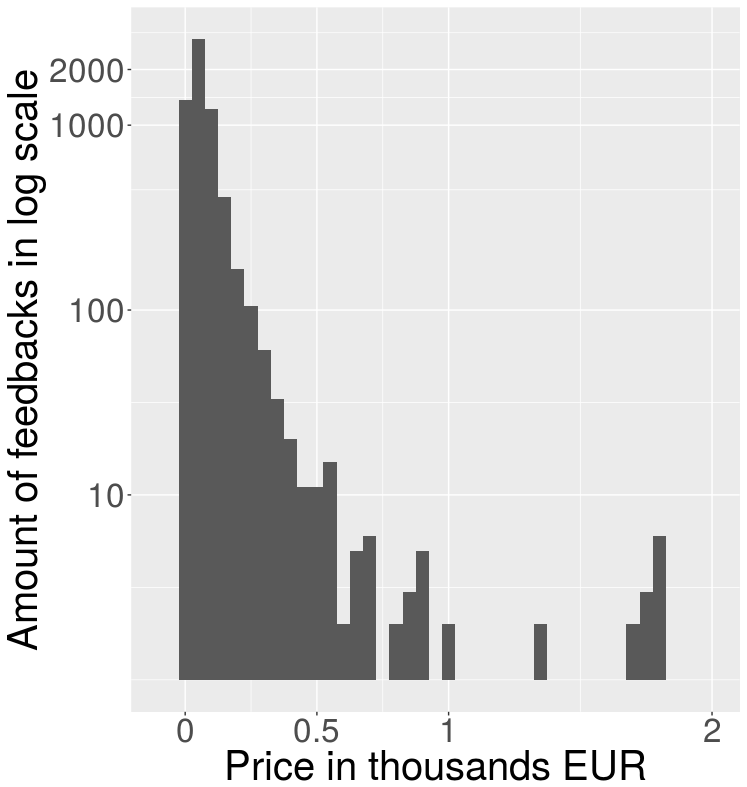
\includegraphics[width=0.5\linewidth]{flistingxprice}
    %\caption{Prices of listings in feedbacks}
    }
    
\caption[justification=centering]{Distribution of prices in listings and feedbacks\newline }
\end{figure}

We calculated the last month revenue for each category
by summing the price over all feedbacks to listings in given category.
This leads to minimal revenue, because feedbacks
can be given only if the trade happened on cryptomarket and 
trades happening with no given feedbacks are also possible.
The total revenue over one month, amount of listigs and feedbacks and market share for given categories 
is in table \ref{categories}.
Market share is a revenue of category divided by total revenue from all categories.
The total revenue over given month was 527730EUR.
Average price of occured trades was similar in each category
with two outliers. Opiates, which have the high price/dose ratio and 
self-defence, which had only 4 trades, 2 of them were custom listings and 2 of them were guns.
Custom listings contains no special tag and no description of any goods/services.
They contain just titles like "custom listing for user: xxx", "custom 013" and so on.
We found 300 listings with word "custom" in their title. 
We think that vendors and buyers use these custom listings in order to be able to protect themselves
by cryptomarket escrow service for already arranged deal.


\begin{table}
    \caption{Estimated monthly revenue for selected drug categories based on feedbacks}
\hspace*{-1cm}
    \label{categories}
    \begin{tabular}{|l|l|l|l|l|l|}
Category & listings & feedbacks &  \multicolumn{1}{|p{2cm}|}{\centering revenue \\ in EUR }& \multicolumn{1}{|p{2cm}|}{\centering average price \\ in EUR } &\multicolumn{1}{|p{2cm}|}{\centering market \\ share } \\
Cannabis & 5139 & 1883 & 135693 & 72 & 27.6\% \\
Stimulants & 3493 & 1043 & 108157 & 103 & 22\% \\
Opiates & 1662 & 489 & 83135 & 170 & 16.9\% \\
Pharmacy & 2294 & 1104 & 62054 & 56 & 12.6\% \\
Body building & 679 & 402 & 31466 & 78 & 6.4\% \\
Empathogens & 2988 & 394 & 20344 & 51 &4.1\% \\
Other drugs &  774 & 173 & 14350 & 82 & 2.9\% \\
Psychedelics & 1377 & 198 & 11796&59  & 2.4\% \\
Other products &  782 & 89 & 9106& 102 & 1.8\% \\
Self-defence &  513 & 4 & 4635 &  1158  & 0.9\% \\
Services & 1662 & 35 & 4061 &  116  &0.8\% \\
Dissociatives &  290 & 38 & 2317& 60  & 0.5\% \\
Classifieds &  649 & 18 & 2182 &  121  & 0.4\% \\
    \end{tabular}
\end{table}


Most of the vendors had listings in just few categories.
The graph \ref{catxrev} shows amount of vendors with given revenue and number of different subcategories they have 
active listings in. Most vendors sell goods just in few categories, hovewer, vendors with 10000EUR or more in
revenue tend to have listings in more categories. The boxchart \ref{boxcat} the distribution of vendors revenue based on category they were
selling in. We have not count vendors with 0 revenue for the boxchart chart. If vendor was selling in multiple categories, we
divided his revenue by the number of categories and counted him in both.

\begin{figure}[!htb]
    \centering
    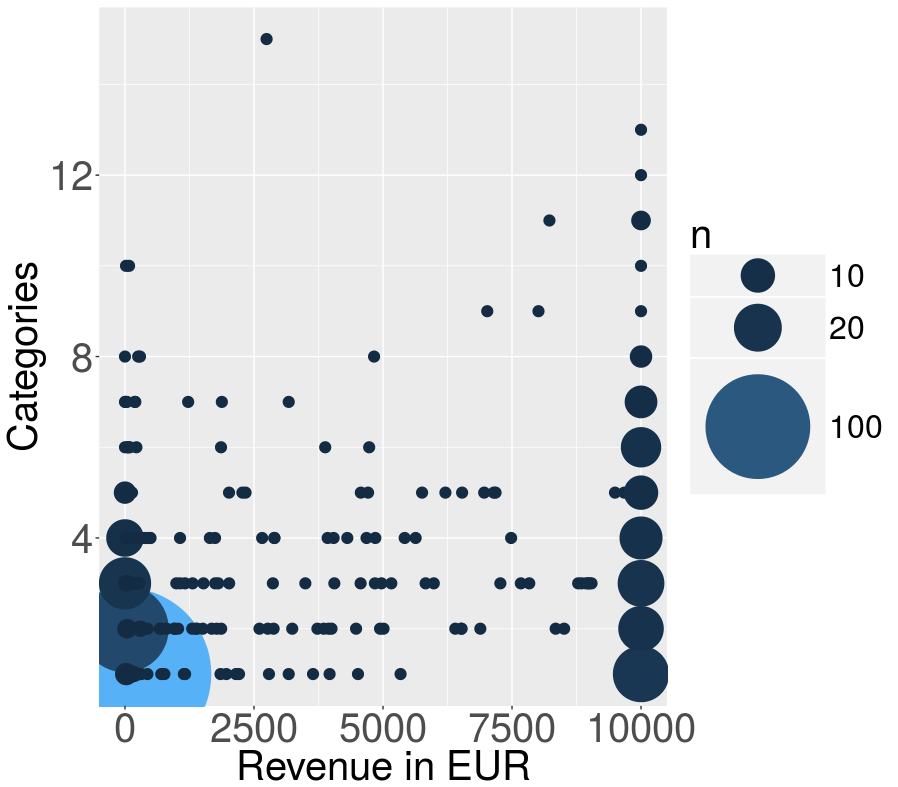
\includegraphics[scale=0.4]{catxrev}
    \caption{Amount of vendors with number of different categories they sell and their total revenue}
    \label{catxrev}
\end{figure}

\begin{figure}[!htb]
    \centering
    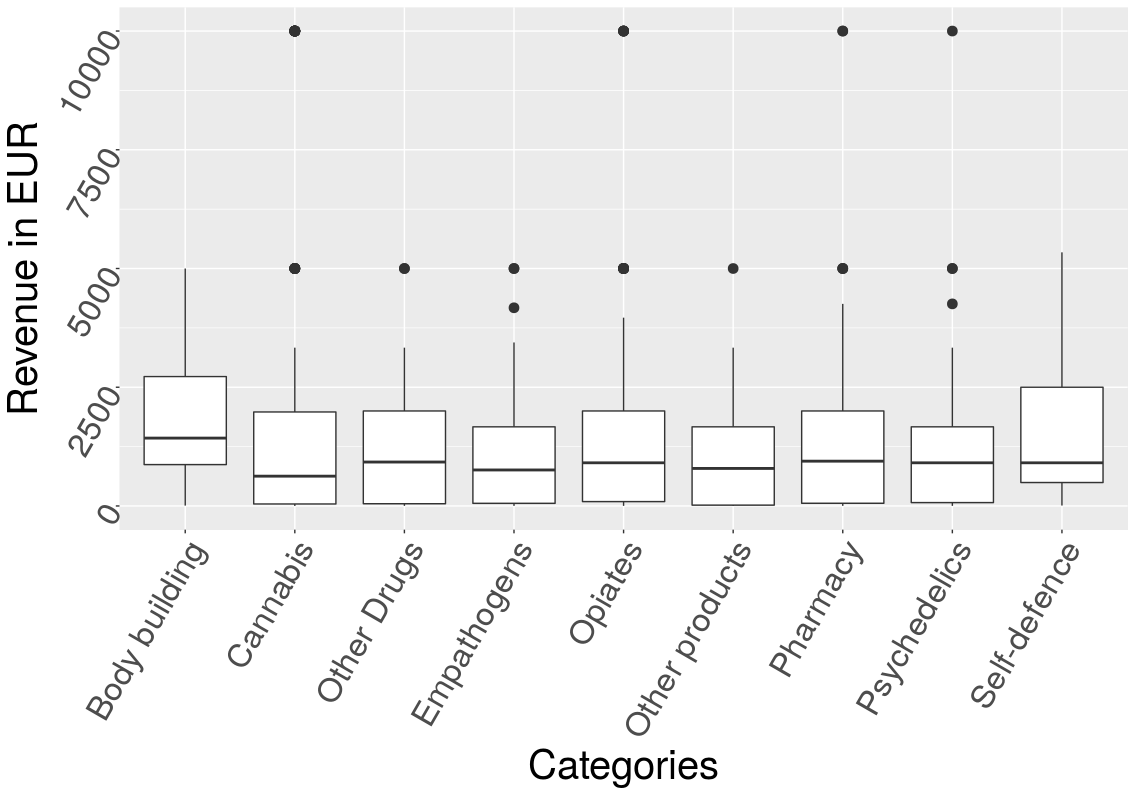
\includegraphics[scale=0.4]{boxcat}
    \caption{How much have Vendors earned based on category they sell}
    \label{boxcat}
\end{figure}


Vendor pages contains counts of feedback gathered over lifetime, these were used
in \ref{posratrev}. Vendors also has feedback pages, where feedbacks younger than
1 month contain first two and last two characters of buyers username,
, the rounded total number and price of trades performed by buyer.
We used these feedbacks to gather informations about buyers.

There are possible $36^4=1679616$ combinations of 4 alfanumerical characters.
From our 6000 feedbacks, we gathered 2433 unique combinations of four letters from username,
when added rounded number of trades and buyer's total spending we got 2654.
It is highly probable that some different buyers have the same username prefix, suffix, amount of 
trades and revenue, because when considering buyers total spending and trades, we managed to increase
the number of identified buyers. Buyers total spending and total performed trades are rounded just to few distinct values, so the
following statistics are just estimates.

Each buyer have bought on average goods for 1176EUR through all his trades on Valhalla market.
Just 129(5\%) of buyers had bought goods with worth rounded to 10000EUR in total,
 1289(50\%) buyers have spendings 500EUR or less.
This distribution is similar to revenue distribution of vendors, where
vast majority of actors transfer just small amounts of value through Valhalla market and
just extremely small percentge of actors trade on market at bigger scale.
The average price of the one trade (82.7 EUR) and the average of lifetime spending (1176EUR)
is way below the amount someone who actively resell drugs for profit would buy.
The distribution of buyers total spending is on figure \ref{buyerxspend}.

\begin{figure}[!htb]
\hspace*{-3cm}
    \label{buyerxspend}
\subfloat{
    \centering
    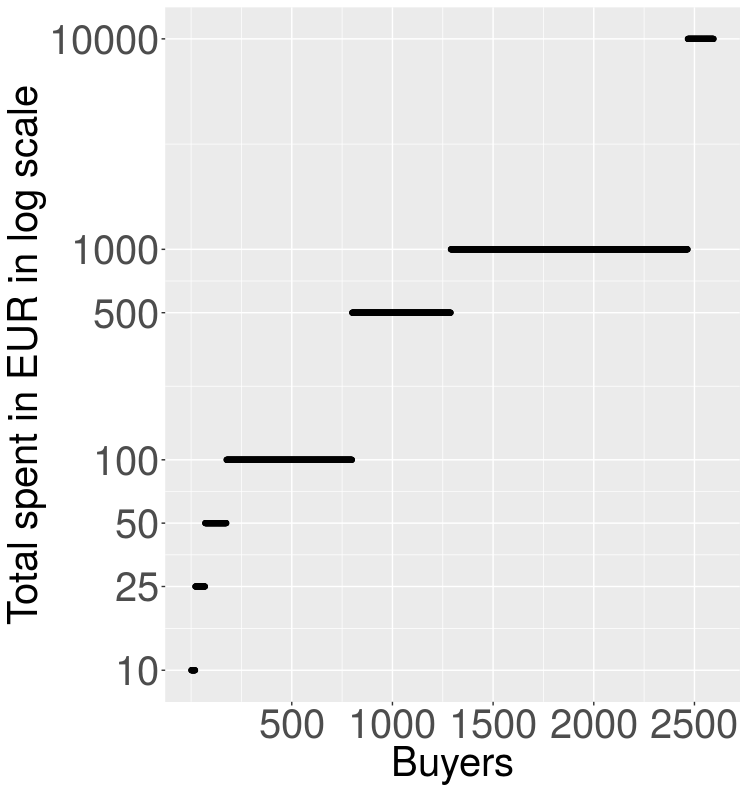
\includegraphics[scale=0.4]{buyerxspend}
    %\caption{Rounded amount the buyers totally spent on Valhalla market}
}
\subfloat{
    \centering
    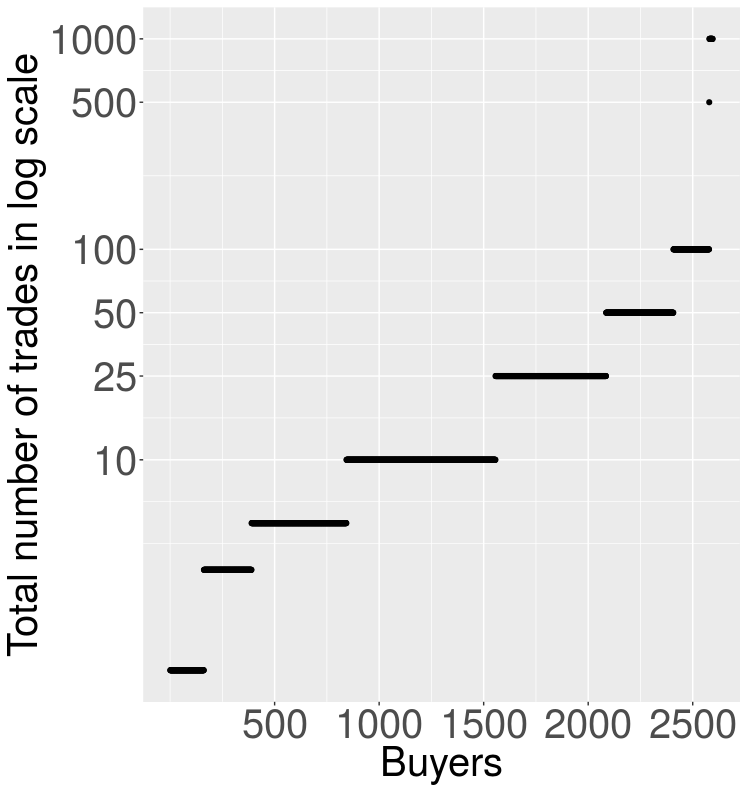
\includegraphics[scale=0.4]{tradxbuyer}
    %\caption{Distribution of total trades}
}
\caption[justification=centering]{Distribution of buyers total spending and total performed trades}
\end{figure}


\chapter{Conclusions and future work}

We were succesfull with scraping Valhalla cryptomarket and
bringing up meaningful and intersting statistics about its vendors and users.
Our statistical findings fits into the previously published desciptions
of cryptomarkets, but we also found some statistics where Valhalla market is outlier and
came up with reasons why is it so.
We scraped Valhalla market once, but the data about the feedbacks were
related to the time frame of one month. Continously monitoring 
Valhalla cryptomarket for longer periods of time could enchance the statistical description
with data about changes of various trends on this market over time.

Our application is fully working and production ready, it 
finds nearest addresses with associated identities for given address.
The application could be extended in multiple ways. We used two
heuristics that have lowest risk of falsely clustering addresses belonging to different identities.
The heuristics have not clustered all the addresses and transactions that have been done by crypto market,
hovewer we found, that with just tens of deposits and withdrawals between us and market,
we were able to identify significant percentage of cryptomarket's cashflow over given month.
The price that we payed in fees in these transaction was alltogether less than 100 dollars. 
Perpetual depositing and withdrawals over prolonged period of time seems financially feasible
and might lead to disclosing majority of cryptomarkets addresses and transaction.

Application could be extended by adding more heuristics for clustering addresses. Some of these
heuristics have been described in \parencite{androulaki2013evaluating}.
These heuristics are not based just on graph of bitcoin transactions, but also
on expected behaviour of users and data that can be obtained by continously running one or multiple
bitcoin nodes. These heuristics are less reliable, but offer more options to cluster addresses of same owner.

The whole application backend can be run on consumer grade notebook. Backend database as indexed and utilizes memory well
, requests from GUI takes at most 30 seconds to complete. This is to application advantage,
hovewer application set up takes long time, for the simple reason that bitcoin
blockchain consists of roughly 150GB of data and these must be inserted into database, indexed
and processed by heuristics.
For setting the application up on server and having users access it remotely,
different options viable for storing and retrieving data on server hardware
(for example in memory database if RAM is big enough can be considered.

\printbibliography

\end{document}
